\documentclass[letterpaper,12pt]{article}
\usepackage{opticameet3}
\newcommand\authormark[1]{\textsuperscript{#1}}

\graphicspath{ {./images/} }
\usepackage[font=footnotesize]{caption}

\usepackage{floatrow}
\usepackage{amsmath,amssymb}
\usepackage{multicol}


\usepackage{listings}
\geometry{letterpaper}
\usepackage{xcolor}

\usepackage{setspace}


\bibliographystyle{unsrt}
\def\bibfont{\footnotesize}

\geometry{left=1in,right=1in,top=1in,bottom=2in}
\hbadness=99999
\tolerance=10000
\setlength{\headheight}{14.49998pt}

\usepackage{fancyhdr} % Include the fancyhdr package
\usepackage{lipsum}   % For dummy text

% Configure the fancyhdr package
\pagestyle{fancy}     % Activate the fancyhdr package

% Clear default header and footer styles
\fancyhf{}


% Set header contents
\fancyhead[L]{\textbf{Monsoon 2024}} % Left-aligned
\fancyhead[C]{\textbf{Honors Report}} % Left-aligned
\fancyhead[R]{\textbf{\thepage}}          % Right-aligned (Page number)


% Define colors for syntax highlighting
\definecolor{codegreen}{rgb}{0,0.6,0}
\definecolor{codegray}{rgb}{0.5,0.5,0.5}
\definecolor{codepurple}{rgb}{0.58,0,0.82}
\definecolor{backcolour}{rgb}{0.97,0.97,0.98}


% Configure Python listing style
\lstdefinestyle{python}{
    backgroundcolor=\color{backcolour},
    commentstyle=\color{codegreen},
    keywordstyle=\color{magenta},
    numberstyle=\tiny\color{codegray},
    stringstyle=\color{codepurple},
    basicstyle=\ttfamily,            % Use tiny font size
    breakatwhitespace=false,
    breaklines=true,
    captionpos=b,
    keepspaces=true,
    numbers=left,
    numbersep=5pt,
    showspaces=false,
    showstringspaces=false,
    showtabs=false,
    tabsize=4,
    frame=single,                    % Add frame around the code
    framesep=2pt,                    % Small frame separation
    framerule=0pt,                 % Thin frame rule
    xleftmargin=10pt,
    xrightmargin=10pt,
    % Python specific settings
    language=Bash,
    morekeywords={self},             % Add self as a keyword
    emph={MyClass,__init__},         % Add custom highlighting for classes
    emphstyle=\color{blue},
}


\date{\today}

\usepackage{xcolor}
\definecolor{violet}{HTML}{3300AD}
\usepackage[colorlinks=true,bookmarks=false,citecolor=blue,urlcolor=blue,linkcolor=violet]{hyperref}
\begin{document}
\begin{spacing}{1.125}

\begin{figure}[!ht]

\includegraphics[width=0.5\textwidth]{iiith_logo.png}
\end{figure}
\vspace{0.5cm}
\title{\Large{Honors Report} \\ \normalsize{Monsoon 2024} \\ \vspace{1cm} \Huge{Introduction to Collision
Simulations and Brief Review on Foundation Models}}
\vspace{1cm}
\author{Abhiram Tilak - 2022113011}
\address{\authormark{*}International Instituite of Information Technology, Hyderabad}
\vspace{1cm}

\begin{abstract}
This report documents efforts to acquire proficiency in tools commonly used for collision
simulations, specifcally Pythia8, and ROOT. The application of these tools is
demonstrated through the execution of sample simulations.

Additionally, the report provides a concise review of foundational models in the field
of high-energy physics, with a particular focus on a paper discussing Masked Particle Modeling.
\end{abstract}

\pagebreak





\tableofcontents
\listoffigures
\lstlistoflistings


\section{Collision Simulations}


A standard method for studying collider physics is to simulate the collisions
of two particles using the computer program PYTHIA and assume that their
interaction is governed by a particular physics model, which can be inserted into
PYTHIA as an input file and generated by yet another program called Mad-
Graph. Performing this simulation repeatedly to achieve a desired statistical
certainty is called a Monte Carlo simulation.

For the sake of sample simulations, we won't be using Mad-Graph and perform
multiple simulations, but perform individual simulations usign Pythia8 and
explore tools like ROOT which help in analyzing the results.

The Pythia program is a standard tool for the generation of high-energy
collisions, comprising a coherent set of physics models for the evolution from a
few-body hard process to a complex multihadronic final state. While previous
versions were written in Fortran, Pythia 8 represents a complete rewrite in
C++.

\subsection{A simple proton collision}

The simulation of the proton-proton collision is a complex procedure that takes
many steps in order to
best reproduce the detector output generated by different physics processes.

The simulation chain can be summarized in three main steps: event generation,
detector simulation
and digitisation. We will be concentrating in the first step here.

The first step in the simulation chain is the generation of all the physics
processes of interest. At this level
the beam collision is treated only as the interaction between two partons of the
protons, described using
specific PDFs.

Below is the Pythia configuration used for the simulation:
\begin{lstlisting}[style=python, caption={Pythia configuration for Sample Simulation}]
    // proton pgp is 2212
    pythia.readString("Beams: idA = 2212");
    pythia.readString("Beams: idB = 2212");
    pythia.readString("SoftQCD:all = on");
    pythia.readString("HardQCD:all = on");
    pythia.init();
\end{lstlisting}

\paragraph{Configuration:}
First, the program initializes the Pythia object and configures it to simulate
collisions between two protons, identified by their Particle Data Group (PDG)
code, 2212. It enables both soft and hard QCD (Quantum Chromodynamics)
processes, which govern how quarks and gluons interact, ensuring a wide range of
collision dynamics. After the setup, the simulation is initialized.

Note that the full source code can be found on my
\href{https://github.com/abhiramtilakiiit/research/blob/main/simulations/introduction/proton_collision.cc}{github}.

\paragraph{Code Explanation:}
The main loop runs for a predefined number of events (n). For each event, Pythia
generates the particles resulting from the collision. If the generation is
successful, the program retrieves and prints the total number of particles in
the event. For each particle, it extracts and displays properties like its
particle ID (a unique identifier for the particle type), its mass, and its
momentum (calculated from its momentum components in the x, y, and z
directions). By analyzing these properties, users can study the physics of the
collisions and the types of particles produced.

The output will show basic information that we have printed out using the
\texttt{cout} commands, like the entry number and other values like momentum and
mass in each iteration. But this output is not the most readable, we have to
use different tools to plot them in graphs or find other programs to analyse and
infer for us.

\subsection{Creating a Histogram:}

Using the \texttt{Pythia8::Hist} object we can create a histogram and plot any
parameter of choice.

To initalize a simple Histogram which plots z-component of momentum (Pz) we add the following command
in the configuration phase:

\begin{lstlisting}[style=python, caption={Initializing Histogram object in Pythia}]
    Pythia8::Hist hpz("Momentum (Pz) Distribution", 100, -10, 10);
\end{lstlisting}

The arguments are 100; which refers to the number of buckets in the histogram.
The -10 and 10 refer to the range of values the histogram should cover. In this
case since we chose 100 buckets from -10 to 10, which have 20 values, each
bucket will have a width of 0.5.

Once the code is compiled and run, the histogram is directly printed out in the
terminal STDOUT shown in figure \ref{graph-text}:

\begin{figure}[!hb]
  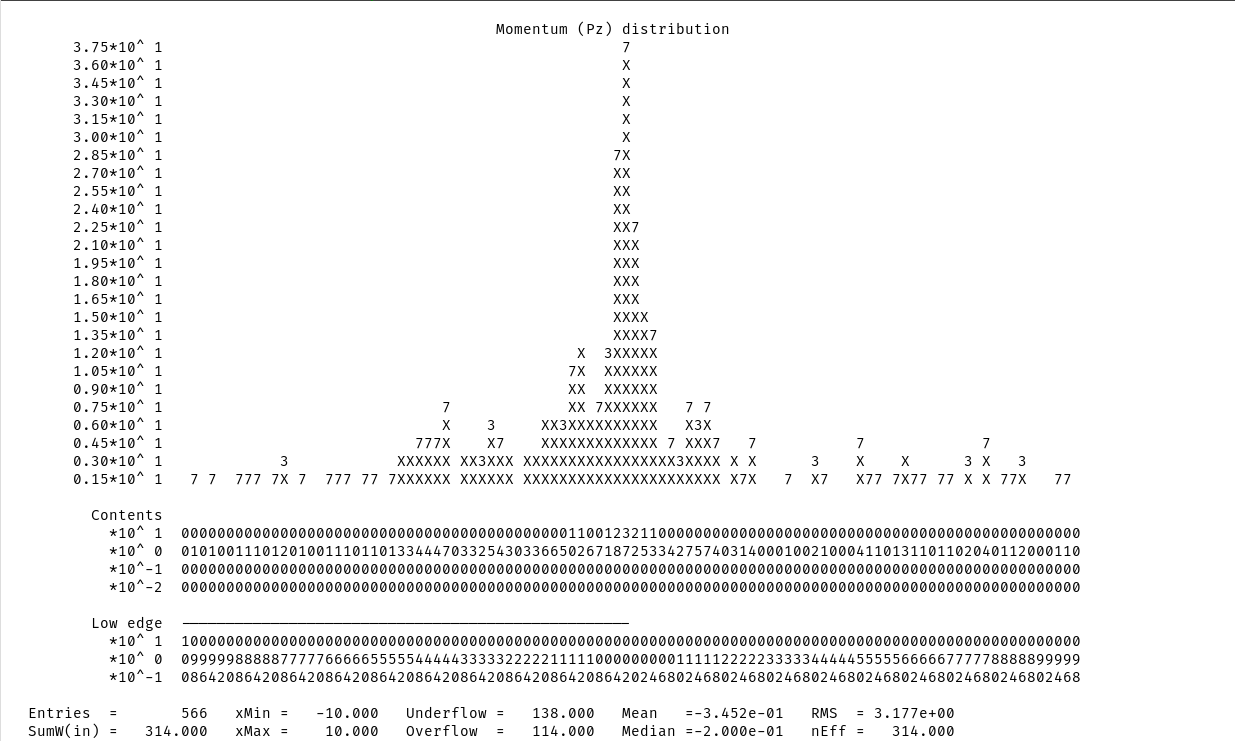
\includegraphics[width=\textwidth]{graph-text.png}
  \caption{ASCII histogram of momentum distribution output by Pythia's Hist tool}
  \label{graph-text}
\end{figure}

From the graph we can make the following inferences:
\begin{itemize}
  \item We have 566 entries, that means 566 particles have been generated in the
    simulation.
  \item The SumW is the Weighted sum of the values in the given graph.
  \item Underflow and Overflow refer to the mininum and maximum values of the
    momentum which are not captured in the graph because of the xMin and xMax
    values, set during configuration.
  \item Both the mean and median are very small values, suggesting more or less
    it is near to zero and is evident because the initial momentum of the beams
    in z-direction is 0.
  \item The RMS shows the root mean square value of the Pz, which should be
    similar to that of the mean of \texttt{P\_abs} which we also print.
\end{itemize}


\paragraph{Using HistPlot and Pyplot: } We can also use pyplot to get a better smoother graph than the ascii one in the
terminal. Note that, using this tool we get a python file along with an output
file, and might need python installed and tools like matplotlib setup for the script to work.

We can configure the HistPlot at the very end after we print out the histogram
as follows:

\begin{lstlisting}[style=python, caption={Configuring Pyplot for Histogram using HistPlot}]
  Pythia8::HistPlot hpl("myhistplot");
  hpl.frame("histout", "Momentum (Pz) Distribution", "Momentum (Pz)", "Entries");
  hpl.add(hpz);
  hpl.plot();
\end{lstlisting}

Now after compiling and running, we see an additional data file and a python
file, which will generate the actual plot in pdf format. The plot can be shown in the figure
\ref{graph-py}

\begin{figure}[!ht]
  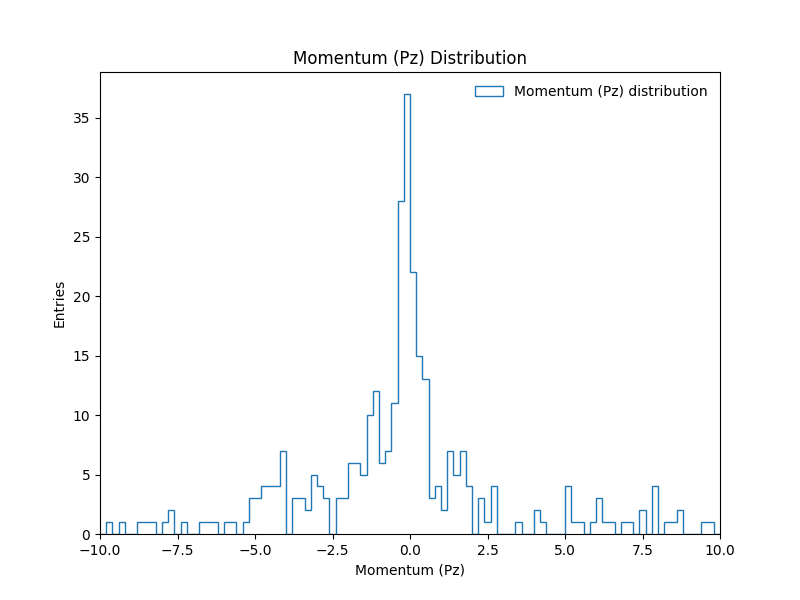
\includegraphics[width=0.6\textwidth]{graph-py.png}
  \caption{PyPlot version of Momentum Distribution Histogram}
  \label{graph-py}
\end{figure}



\subsection{Root Trees and Histogram}


ROOT is a software framework for data analysis and I/O: a powerful tool to cope with the
demanding tasks typical of state of the art scientific data analysis. Among its prominent
features are an advanced graphical user interface, ideal for interactive analysis, an
interpreter for the C++ programming language, for rapid and efficient prototyping and a
persistency mechanism for C++ objects, used also to write every year petabytes of data
recorded by the Large Hadron Collider experiments. This introductory guide illustrates
the main features of ROOT which are relevant for the typical problems of data analysis:
input and plotting of data from measurements and fitting of analytical functions.

ROOT provides myriad of tools for data analysis, but In this sample analysis we will be focussing in root trees
using the \texttt{Ttree} tool.

A TTree behaves like an array of a data structure that resides on storage -
except for one entry (or row, in database language). That entry is accessible in
memory: you can load any tree entry, ideally sequentially. You can provide your
own storage for the values of the columns of the current entry, in the form of
variables. In this case you have to tell the TTree about the addresses of these
variables; either by calling TTree::SetBranchAddress(), or by passing the
variable when creating the branch for writing. When “filling” (writing) the
TTree, it will read the values out of these variables; when reading back a TTree
entry, it will write the values it read from storage into your variables

\subsubsection{Configuring TTree}

Configuration of the root tree, involves initializing the TFile file-system, and
initializing the TTree object. We create different variables which are to be
written, and create a new branch corresponding to each of the variables:

\begin{lstlisting}[style=python, caption={Configuration of Root TTree in Pythia}]
    // TFile setup - First argument is the name of the file/tree
    TFile *output = new TFile("root_tree.root", "recreate");
    TTree *tree = new TTree("tree", "tree");

    int id, event, size, no;
    double m, px, py, pz;

    // Initialize tree branches
    tree->Branch("event", &event, "event/I");
    tree->Branch("size", &size, "size/I");
    tree->Branch("no", &no, "no/I");
    tree->Branch("id", &id, "id/I");
    tree->Branch("m", &m, "m/D");
    tree->Branch("px", &px, "px/D");
    tree->Branch("py", &py, "py/D");
    tree->Branch("pz", &pz, "pz/D");
\end{lstlisting}

Again please consult the full source code before I try to explain some
components:

\paragraph{Explanation} In the main loop for every successful event, the total number of particles (n\_particles) produced in the
collision is retrieved. The program iterates through all these particles, extracting their
properties such as particle ID (id), mass (m), momentum components (px, py, pz), and the
particle's index (no) within the event. Each particle’s data is then stored in a TTree—a
ROOT data structure designed for efficient storage and retrieval of structured data.
The tree->Fill() command writes these properties for each particle into the TTree.

Once all events are processed, the output file is written to disk using output->Write(),
and the file is closed. The resulting ROOT file can then be analyzed further, allowing
physicists to study particle properties, kinematics, and distributions resulting from the
simulated collisions.

\subsubsection{Analysing the ROOT File}

After running and compiling the above cpp file, a new root file is created. To
analyse it we open it with the root command (\texttt{root output.root}).

The first step is to check if our root tree is filled with all the required
information. We can get access to an ascii-table with all the recorded info
using the Scan() function, the output can be found in the figure \ref{table}

We can then open the root file-system corresponding to the file and browse
through it by spawning a TBrowser instance. (\texttt{new TBrowser}).


\begin{figure}[!ht]
  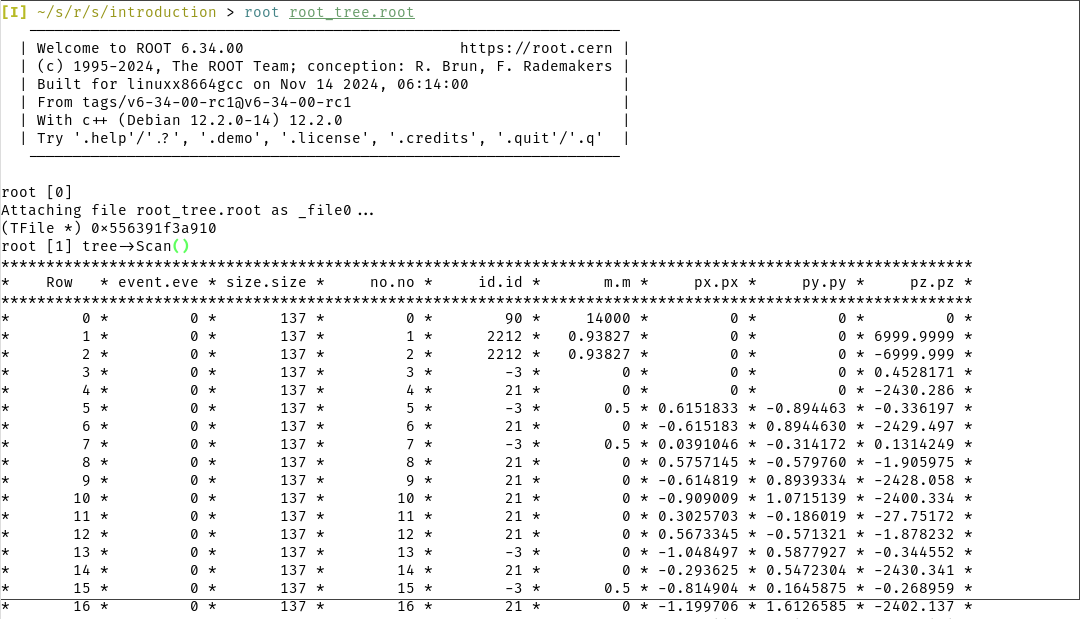
\includegraphics[width=0.8\textwidth]{table.png}
  \caption{Tabulated values recorded in simulation into the TTree}
  \label{table}
\end{figure}


The file directory should contain the tree that we plotted and different
branches are the paramaters. Just by double clicking, we can obtain a histogram
of that paramter. Some limits in the histogram need adjusting because the
defaults are usuallly high, but can be adjusted by mouse scroll.

Figure \ref{size-hist} and \ref{pz-hist} show some screenshots of the TBrowser
in action.

\begin{figure}[!ht]
  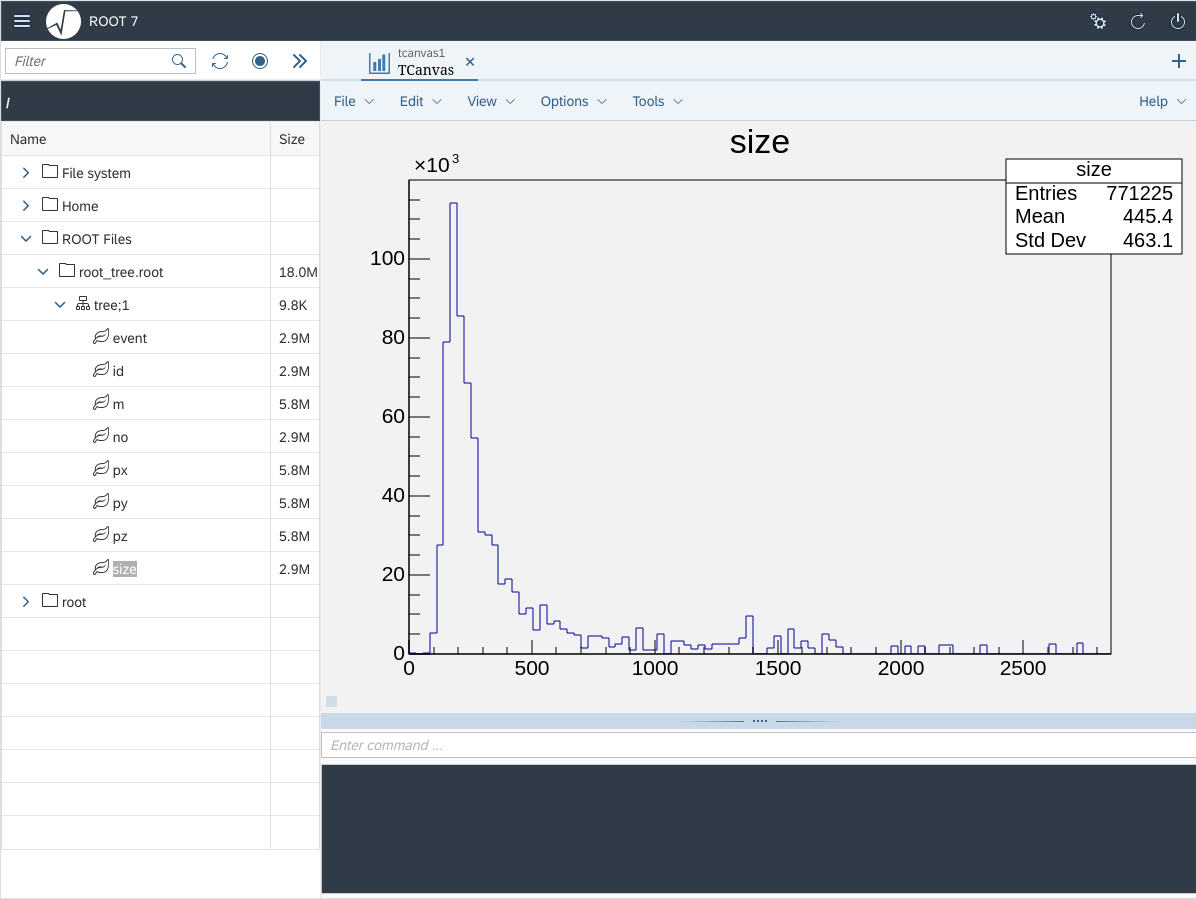
\includegraphics[width=0.8\textwidth]{size-hist.png}
  \caption{Histogram for size (number of particles in an event) in TBrowser}
  \label{size-hist}
\end{figure}

\begin{figure}[!ht]
  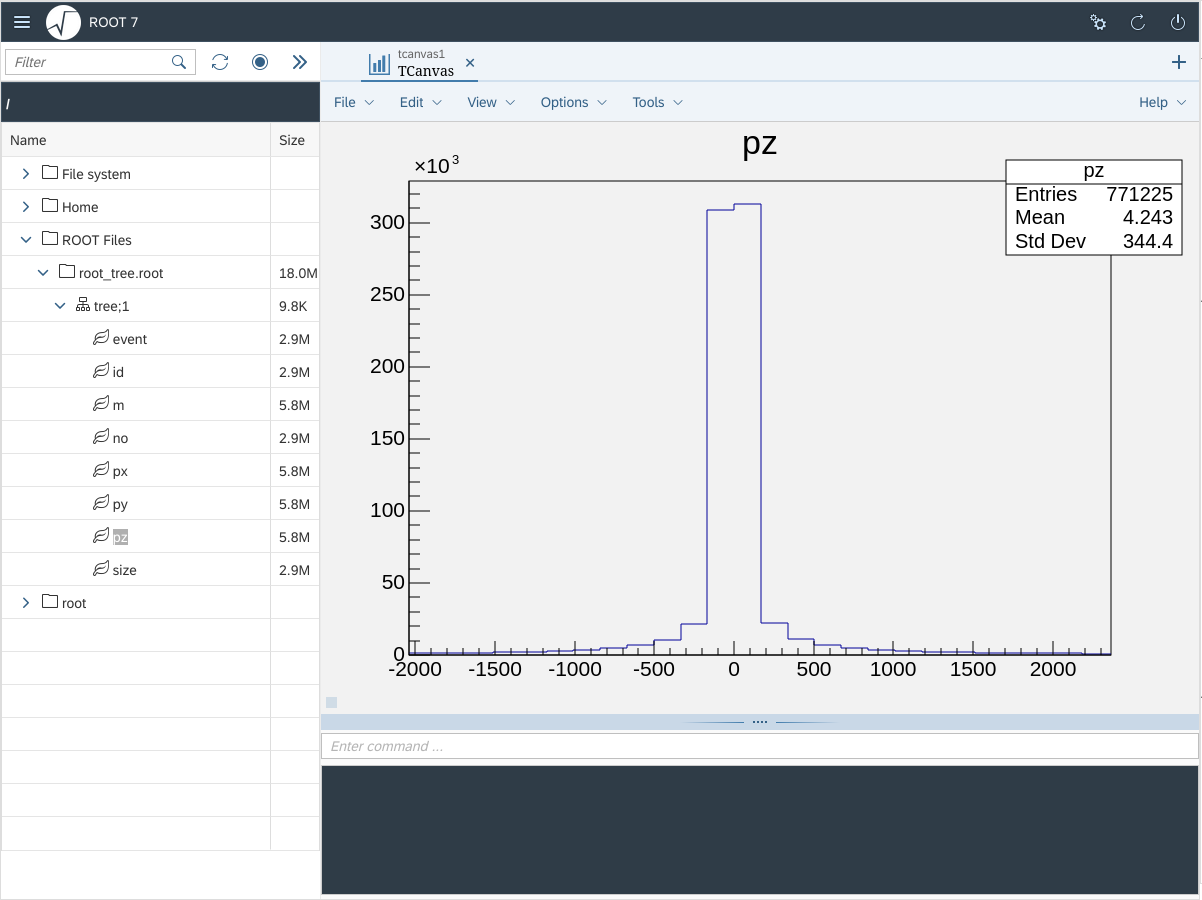
\includegraphics[width=0.9\textwidth]{pz-hist.png}
  \caption{Histogram for Pz (Momentum in Z-direction) in TBrowser}
  \label{pz-hist}
\end{figure}


\subsubsection{Creating a custom Histogram for Analysis}

We can use the Draw() tool to draw, a specific Histogram with a given
condition. The condition can be passed as a second paramter to the Draw command
along with the original paramter on which condition is placed. Example:


\begin{lstlisting}[style=python]
root [1] tree->Draw("m", "id == 2224")
\end{lstlisting}

This will create a histogram for mass (m) for the particle with id (pdb id) as
2224. The resultant histogram can be found in the figure \ref{m-hist}.
The
output from this histogram can also be stored and passed around to other tools
like Geant4.

\clearpage

\begin{figure}[!htb]
  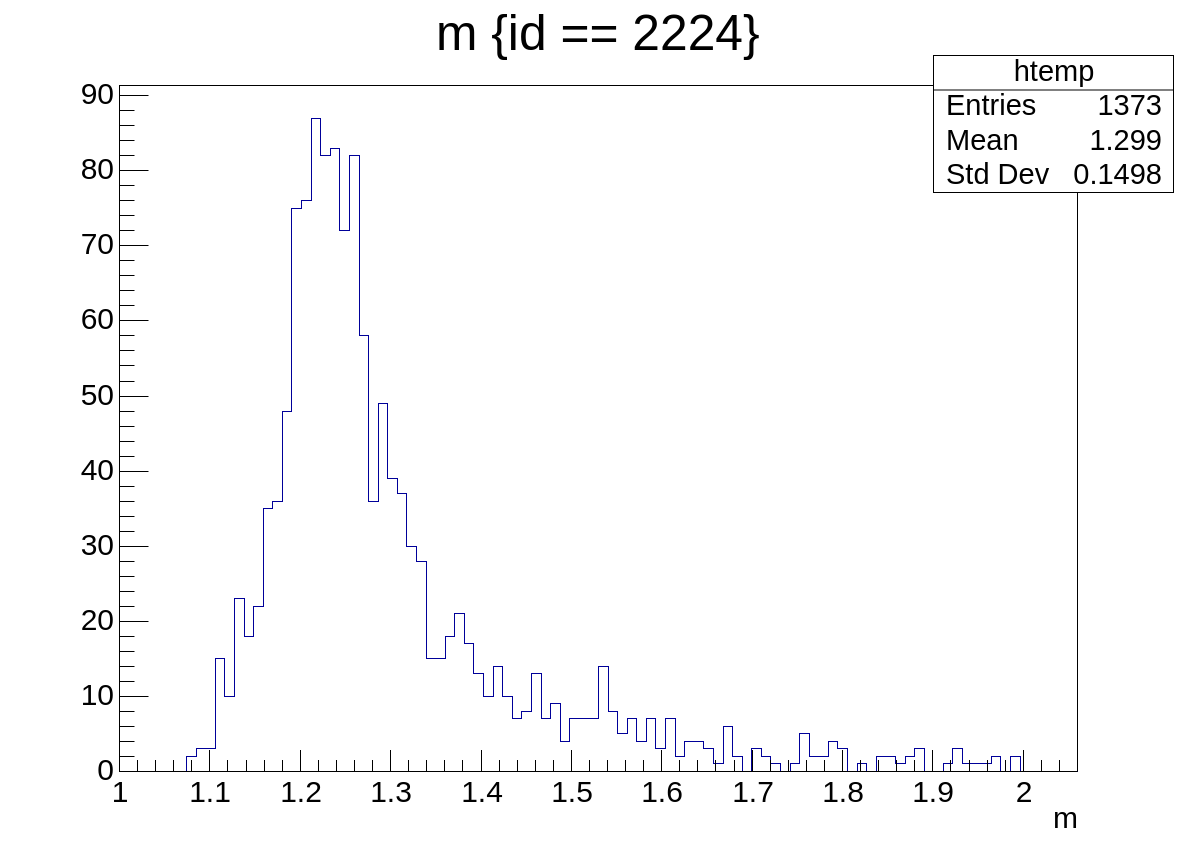
\includegraphics[width=0.9\textwidth]{m-hist.png}
  \caption{Histogram for Mass for particle id == 2224 ($\Delta^{++}$), created
  using the Draw() tool}
  \label{m-hist}
\end{figure}


\pagebreak
\section{Foundation Models}

\footnote{\textbf{Note:} Most of the contents of this part are a subset of ones given in the
\href{https://github.com/abhiramtilakiiit/research/blob/main/presentations/fm.pdf}{presentation}.
Do excuse the fact that this part is presented less as a report but more like presentation, because the
contents are derived from there.
}
Foundation models are multi-dataset and multi-task machine
learning methods that once pre-trained can be fine-tuned for a
large variety of downstream applications.

The aim of this report is to briefly summarize the state of the art of
Foundation models and rapidly increasing amount of research coming out in
the field of particles physics.
There are maily three popular methods in building Foundation models which are popular
in other fields:

\begin{itemize}
  \item Contrastive Learning Methods
  \item Generative Methods
  \item Masking Strategies
\end{itemize}

This report addresses all major adaptations of above models that are found to
date.

\subsection{Foundation Models in Other Fields}

Foundation models are recent developments in artificial intelligence (AI). Models
like GPT 4, BERT, DALL-E 3, CLIP, Sora, etc., are at the forefront of the AI revolution.
While these models may seem diverse in their capabilities – from generating human-like
text to producing stunning visual art – they share a common thread: They are all
pioneering examples of foundation models.

The figure \ref{timeline} shows a timeline chart on popular foundation
models, divided based-on various fields in which they are used.

\begin{figure}[!ht]
  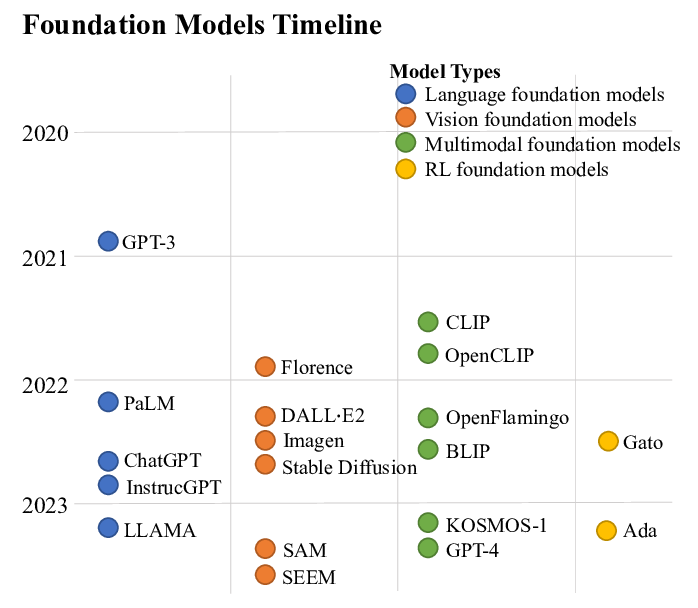
\includegraphics[width=0.7\textwidth]{timeline.png}
  \caption{Foundation Models Evolution Timeline}
  \label{timeline}
\end{figure}

These models are trained on vast amounts of unlabeled or self-supervised data to acquire a
broad knowledge base and language understanding capabilities. They extract meaningful
features and patterns from the training data and fine-tune them for specific tasks.

\paragraph{Why Self-Supervised?}

Self-supervised learning enables foundation models to be trained on vast amounts of unlabeled data without requiring expensive human-annotated labels

Foundation models aim to learn generalized representations that capture
intrinsic semantic structures in data. This is more effectively achieved through
self-supervised learning. Self-supervised objectives create labels directly from the input data, allowing the model to learn meaningful representations without explicit human supervision.


\subsection{Contrastive Learning}


Contrastive Learning is a machine learning technique that teaches computers to understand similarities and
differences by comparing pairs of data points. Similar things should be close together in the computer’s
understanding, while different should be apart

The process involves three main steps:

\begin{itemize}
  \item \textbf{Data Augmentation:} Data augmentation involves applying various transformations to generate diverse versions of the input data. Techniques like cropping, flipping, rotation, and color adjustments are used to create augmented views of the same instance. This increases the dataset's variability and exposes the model to different perspectives of the same data, helping it learn more robust representations.

  \item \textbf{Feature Extraction:}
The encoder network takes the augmented inputs and maps them to a latent representation space. This network learns to extract high-level features and similarities from the data, enabling discrimination between similar and dissimilar instances. Typically implemented as a deep neural network like a CNN for images or RNN for sequences, the encoder captures abstract representations that are useful for downstream tasks.

\item \textbf{Projection:} The projection network transforms the encoder outputs into a lower-dimensional embedding space. This step helps reduce data complexity and redundancy by mapping the representations to a more compact space. The projection enhances the model's ability to distinguish between similar and dissimilar instances, improving overall discriminative power of the learned representations.

\end{itemize}

Figure \ref{clr} gives a good overview of SIMClr model specifically, but can be
generalized to any contrastive learning process.

\begin{figure}
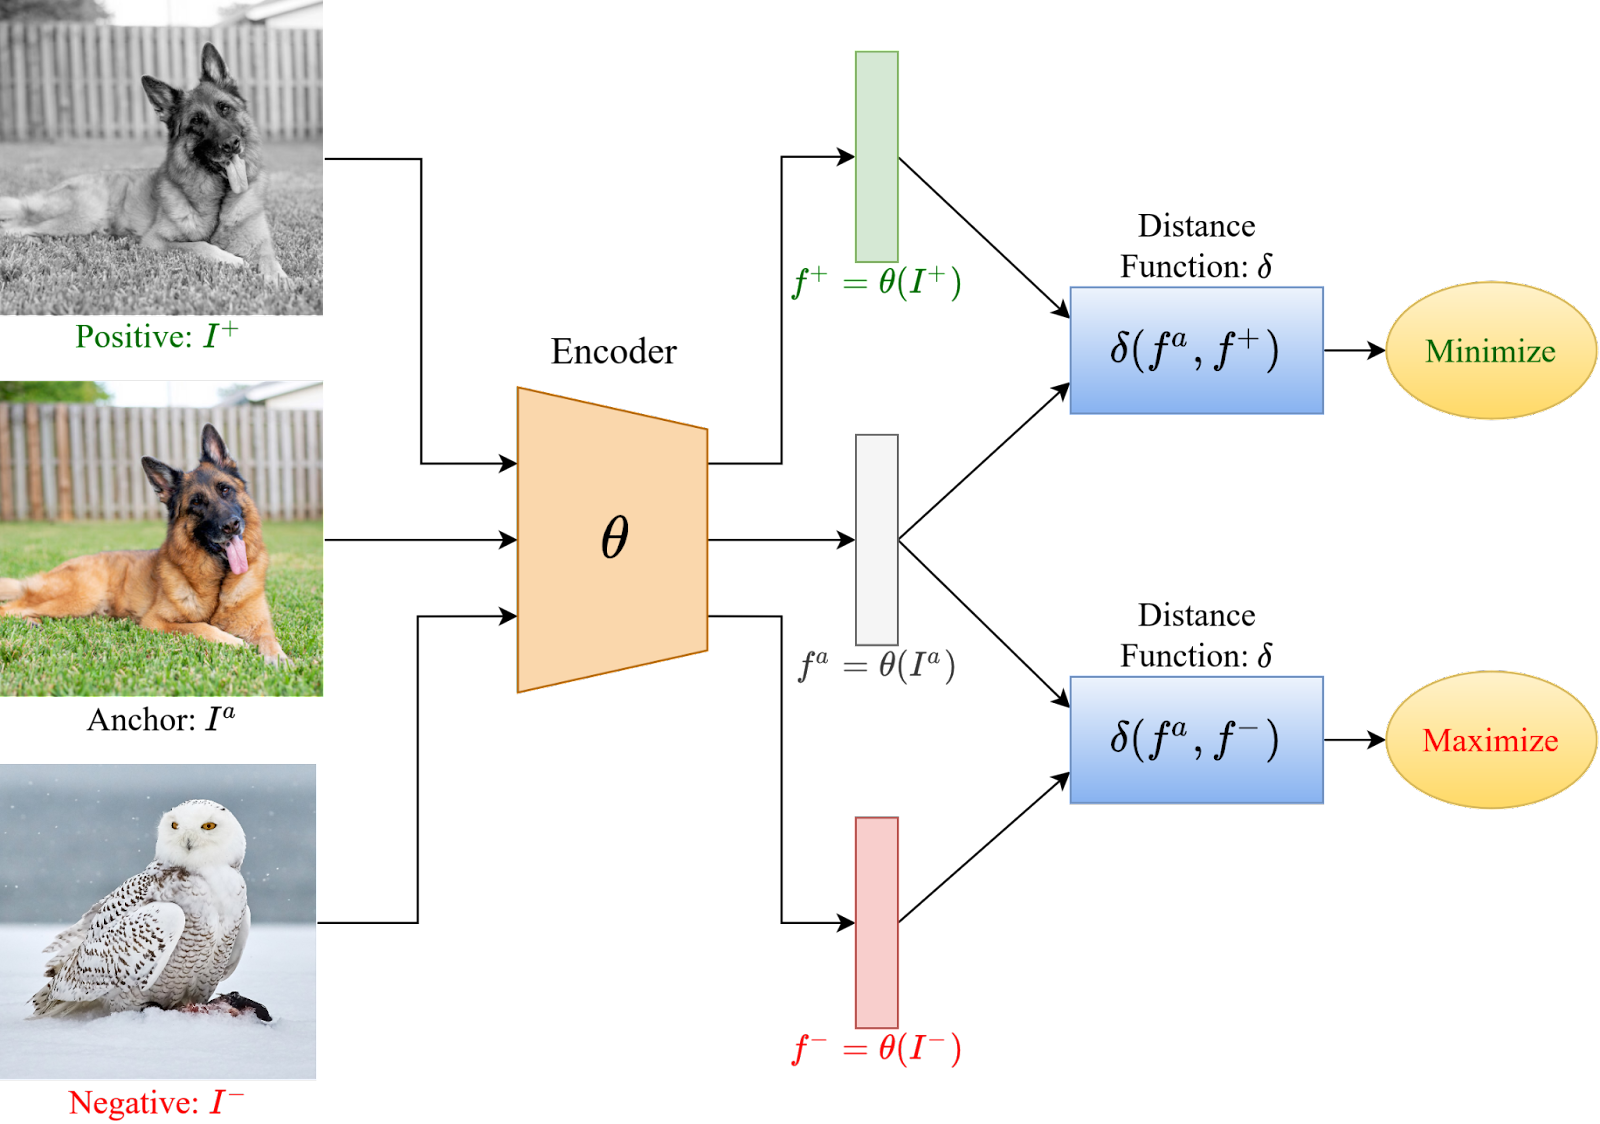
\includegraphics[width=0.8\textwidth]{clr.png}
  \caption{Overview model of contrastive learning}
  \label{clr}
\end{figure}

\subsubsection{Popular Models}

Some popular models based on contrastive learning include:

\begin{itemize}
  \item \href{https://arxiv.org/abs/1911.05722}{MoCo (Nov 2019) (Momentum
    Contrast for unsupervised Visual Representation Learning):}

MoCo treats contrastive learning as a dynamic dictionary lookup process using two encoders - a
query encoder and a momentum encoder - achieving 60.6\% accuracy with ResNet-50 and scaling
up to 68.6\% with R50w4×, making it competitive with larger models while using standard
architectures.
\item \href{https://arxiv.org/abs/2002.05709}{SimCLR (Feb 2020) (A simple framework for contrastive learning of
  visual representation):}

SimCLR is a simplified framework for self-supervised visual learning that outperforms previous
methods by data augmentations and non-linear transformations, achieving 76.5\% accuracy with
linear classifier and 85.8\% on fine-tuned on ResNet-50.

\item \href{https://arxiv.org/abs/2103.00020}{CLIP (Feb 2021) (Contrastive Language-Image Pre-training)}

CLIP (Contrastive Language-Image Pre-training) pairs images with their text captions using dual
encoders (ViT for images, text encoder for captions), matching images to their descriptions in a
shared embedding space, achieving notable zero-shot capabilities in image classification tasks
when trained on 400M image-text pairs
\end{itemize}


\subsubsection{Adaptations of Contrastive learning Models}
Three notable adaptations have emerged in recent years:
\begin{itemize}
  \item \href{https://arxiv.org/abs/2108.04253}{JetCLR (August 2022)}

JetCLR represents a significant innovation in particle physics applications of contrastive learning. This adaptation focuses on creating symmetry-aware representations for jets, emphasizing built-in physical symmetries such as rotation, translation, and permutation. Additionally, JetCLR incorporates soft/collinear safety considerations, addressing potential issues in jet reconstruction. The approach utilizes a transformer-encoder network architecture and evaluates performance through linear classifier tests, demonstrating its effectiveness in distinguishing between different jet configurations.

\item \href{https://arxiv.org/abs/2312.03067}{Dark CLR (October 2024)}

Dark CLR marks a crucial advancement in the quest to detect semi-visible jets from dark sector models. This adaptation leverages contrastive learning with "anomalous enhancements" specifically designed for dark sector physics. By combining representation learning with a normalized autoencoder, Dark CLR enhances its ability to identify subtle anomalies indicative of dark matter signatures. This approach represents a significant step forward in the pursuit of understanding beyond-standard-model physics at the Large Hadron Collider.

\item \href{https://arxiv.org/pdf/2301.04660}{AnomalyCLR (August 2024)}

AnomalyCLR presents a more generalized approach to model-agnostic anomaly detection at the Large Hadron Collider. This adaptation introduces "anomaly-augmentations" that mimic generic features of anomalous events, such as high multiplicity, large missing transverse energy (MET), and large transverse momentum (pT). The method employs a two-step process: contrastive learning followed by an autoencoder applied to the learned representations. This approach demonstrates versatility in detecting a wide range of potential anomalies across various physics scenarios.

\end{itemize}
Another honorable mention is \href{https://arxiv.org/abs/2403.07066v1}{RS3L}
(March 2024) which employs a method of
re-simulation to drive
data augmentation for contrastive learning

\subsection{Generative Models}

A generative model is a type of machine learning model that aims to learn underlying patterns or
distributions of data to generate new, similar data.
This is often used in the context of enabling computers to understand the real world.

Generative models can be both probabilistic or Neural Network based. Figure
\ref{generate} shows the overview of processes in training a probabilistic generative
model.

\begin{figure}[!htb]
  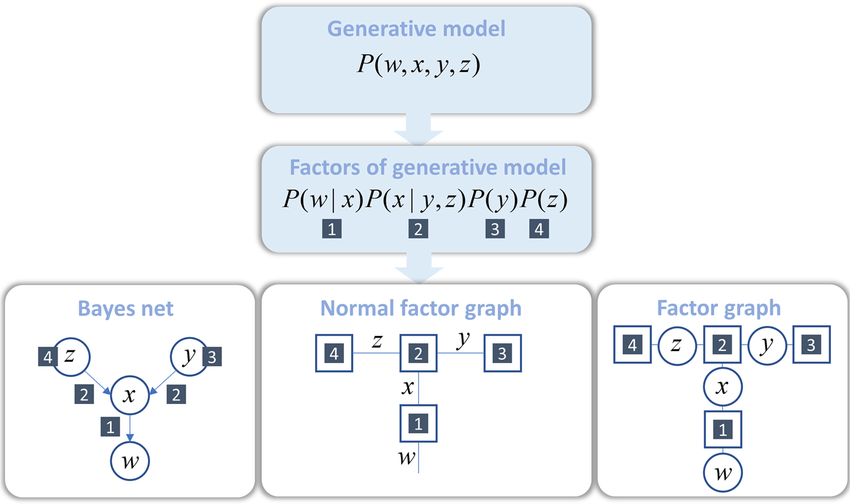
\includegraphics[width=0.8\textwidth]{generative.png}
  \caption{A graphical representation of a probabilistic model.}
  \label{generate}
\end{figure}

Currently generative models
can generate:
\begin{itemize}
\item Images ( Dalle, Stable Diffusion, MidJourney)
\item Text Generation (LLaMA, GPT, Mistral)
\item Audio and Music (WaveNet, BachBOt)
\end{itemize}

There are still efforts to generate Video content through models like SORA
(OpenAI), but the current results are questionable and not promising.

Generative models are too broad of a topic.
We can cover some of the popular approaches and
efforts in adapting them to physics

\subsection{Adaptations of Generative Models}

\begin{itemize}
  \item \href{https://arxiv.org/abs/2202.03772}{ParT (Particle Transformer)
    (July 2023) :}

ParT is based on the traditional Transformer architecture and a successor to ParticleNet, but introduces a modified
attention mechanism specifically for jet tagging. Its major innovation is adding a new term to capture pairwise particle
interactions within the attention mechanism. The model processes jets as particle clouds (unordered, variable-sized sets
of outgoing particles) and was trained on the massive JETCLASS dataset, which is significantly larger than previous
datasets. ParT's training approach is straightforward supervised learning for jet classification, contrasting with more
complex pre-training strategies.

\textbf{Note:} There is a new model MiParT which is works and in version 3, which accommodates the More-Interaction Attention
(MIA) mechanism.

\item \href{https://arxiv.org/abs/2403.05618}{OmniJet (Mar 2024):}
OmniJet is based on the GPT but adapted for continuous physics data. The model's key innovation is its tokenization
strategy for converting continuous particle physics data into discrete tokens, expanding the codebook size to 8192 tokens
(up from 512 in previous approaches). Unlike ParT's direct classification approach, OmniJet first trains in an unsupervised
manner to generate jets as tokens, following the successful pre-training paradigm of language models. The model
demonstrates transfer learning capabilities, where the knowledge gained during generative pre-training can be applied to
downstream classification tasks. Finally, OmniJet aims to be a foundation model for multiple jet physics tasks, contrasting
with ParT's focus on classification specifically
\end{itemize}

\subsection{Dynamic Masking}

Dynamic masking means that the process of selecting and masking words within a sentence is not the same for every epoch during the pretraining phase. This introduces randomness into the training process, and different subsets of words are masked in each epoch. The idea behind dynamic masking is to encourage the model to learn more robust and contextual representations of words.

Such strategies are found in fields like Next Word Predictors which are used in
autocorrects in google keyboards, etc. They use the framework called Masked
Language Model (or general Masked Token Prediction). Popular models like
\href{https://arxiv.org/abs/1810.04805}{BERT}
and \href{https://arxiv.org/abs/1907.11692}{RoBERTa} use this method.

There is also a popular computer vision adaptation, which use Masked
Auto-Encoding strategy (MAE).
MAE is a self-supervised learning technique that masks (removes) portions of an
image and
learns to reconstruct them.

\begin{itemize}
  \item Randomly masks a very high portion of image patches
(typically 75%)
\item Uses much higher masking ratio than NLP because
images have more redundant information
\item This forces the model to understand the overall image
context rather than just copy nearby pixels
\end{itemize}

The figure \ref{mae} goes over a high level overview on the masking strategy
used.


\begin{figure}[!htb]
  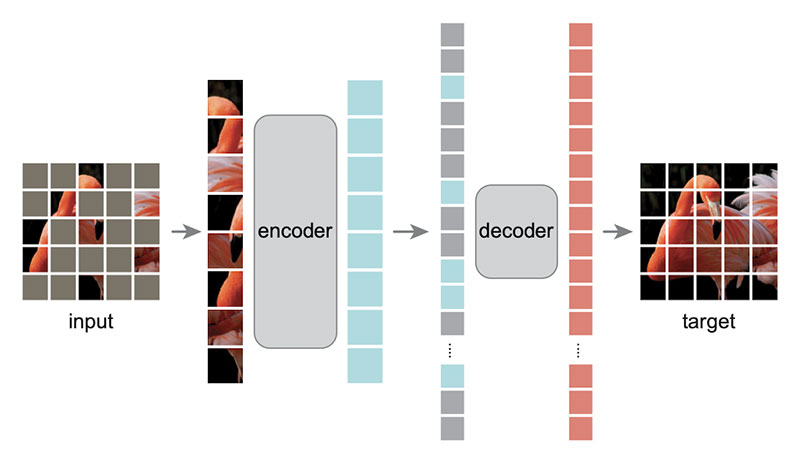
\includegraphics[width=0.7\textwidth]{mae.jpeg}
  \caption{MAE architecture}
  \label{mae}
\end{figure}

In next section discusses a brief overview particular paper which can be seen as
an effort to adapt MLM into High energy physics.

\pagebreak
\section{Masked Particle Modelling}


% ------------------------------------------------------
\end{spacing}
\end{document}

\pagebreak
\section{Foundation Models}

\pagebreak
\section{Masked Particle Modelling}


% ------------------------------------------------------
\end{spacing}
\end{document}
